\documentclass{article}
\usepackage[utf8]{inputenc}

\usepackage{amsthm,amssymb,amsmath}
\usepackage{graphicx}
\usepackage{float}

\newcommand{\NN}{\mathbb{N}}
\newcommand{\ZZ}{\mathbb{Z}}
\newcommand{\RR}{\mathbb{R}}
\newcommand{\QQ}{\mathbb{Q}}
\newcommand{\CC}{\mathbb{C}}

\title{AERO7970 - Trajectory Optimiztion \\ {\small Project 02}}
\author{Matt Boler}
\date{\today}

\begin{document}

\maketitle

\begin{abstract}
  This report presents a solution to a mixed-integer resource allocation problem.
  The solution was implemented in \texttt{Matlab} using the \texttt{intlinprog} solver.
\end{abstract}

%%
\section{Problem Modeling}

We model the solution to the allocation problem as a $1000 \times 12$ binary matrix $X$, where each row is a 1-hot vector $[0, \dots, 1, \dots, 0]$ indicating which station the asteroid is allocated to.
Letting $A$ be the $1000 \times 12$ asteroid-station-mass matrix given in the problem, the asteroid mass at station $i$ can be calculated as
\[
  M_i = A[:, i]^T \cdot X[:, i]
\]

Additionally, maximizing the minimum station mass is not itself a linear objective, so instead we introduce a scalar $S$ representing the lower bound of station masses and maximize it.
This results in the optimization problem:

\begin{align*}
  \max_{X, S} \quad & 10^{-10} * S \\
  \textrm{s.t.} \quad & sum(X(i, :)) = 1 \\
  & A[:, i]^T \cdot X[:, i] \geq S
\end{align*}

\section{Results}

After running the solver, we arrive at the station masses shown below in Figure \ref{fig:masses}.

\begin{figure}[H]
  \centering
  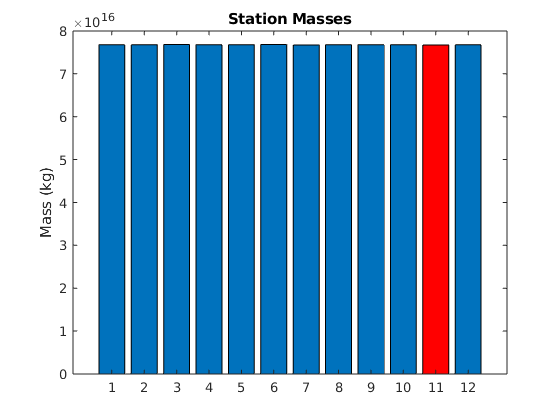
\includegraphics[width=0.7\textwidth]{images/masses.png}
  \caption{Allocated masses for each station}
  \label{fig:masses}
\end{figure}

Station 11 was determined to have the minimum final mass of $7.6750055125e+16kg$, resulting in a final cost $J = 7675005.5125$.
Figure \ref{fig:solver} below shows the progress of the solver over time.

\begin{figure}[H]
  \centering
  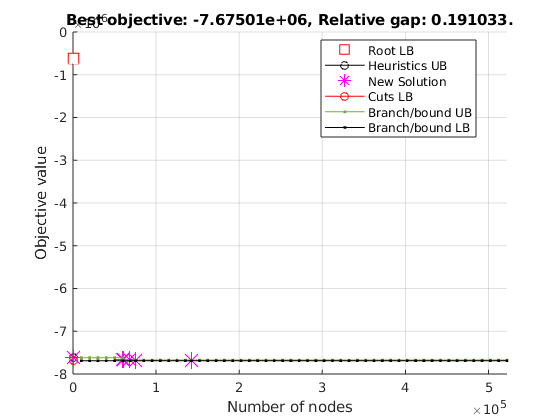
\includegraphics[width=0.7\textwidth]{images/optimizer.png}
  \caption{Solver progress}
  \label{fig:solver}
\end{figure}

\section{Conclusion}

The main challenges of this project were in figuring out how to model the problem and how to get \texttt{Matlab} to actually solve it.
I spent a lot of time trying to find an elegant way to have $X$ be a vector and write the entire system as an $AX = B$ form before deciding on the selection-matrix form.
The fact that these optimization solvers allow fairly arbitrary variable declarations as long as they can be used linearly is a lifesaver.
As for solving the problem, \texttt{intlinprog} is \textit{extremely} slow to solve the problem so I took a lot of time tuning the solver options to try and speed it up.

I spent approximately 15 hours on this project.

\end{document}
